% Cortex - Brussels North-South junction: data, SOTA, Phase 0
% Build:  latexmk -pdf phase0_report.tex     (or: pdflatex phase0_report.tex x2)
% Figures come from: python analysis/phase0/step4_figures.py
\documentclass[aspectratio=169,10pt]{beamer}

\usepackage[utf8]{inputenc}
\usepackage[T1]{fontenc}
\usepackage{lmodern}
\usepackage{booktabs}
\usepackage{graphicx}
\usepackage{xcolor}
\usepackage{tikz}
\usetikzlibrary{arrows.meta, positioning}

\graphicspath{{figures/}{../../data/phase0/figures/}}

% ---- palette (matches the figures: validated categorical slots 1-3) ---------
\definecolor{surface}{HTML}{FCFCFB}
\definecolor{ink}{HTML}{0B0B0B}
\definecolor{ink2}{HTML}{52514E}
\definecolor{ink3}{HTML}{8A8880}
\definecolor{cblue}{HTML}{2A78D6}
\definecolor{corange}{HTML}{EB6834}
\definecolor{caqua}{HTML}{1BAF7A}
\definecolor{cgrid}{HTML}{E3E2DD}

\usetheme{default}
\usecolortheme{default}
\setbeamercolor{background canvas}{bg=surface}
\setbeamercolor{normal text}{fg=ink}
\setbeamercolor{frametitle}{fg=ink, bg=surface}
\setbeamercolor{structure}{fg=cblue}
\setbeamercolor{alerted text}{fg=corange}
\setbeamerfont{frametitle}{size=\large, series=\bfseries}
\setbeamertemplate{navigation symbols}{}
\setbeamertemplate{itemize items}[circle]
\setbeamertemplate{footline}{%
  \hfill\usebeamerfont{date}\color{ink3}\scriptsize\insertframenumber\hspace{2em}\vspace{1ex}}

\newcommand{\srcnote}[1]{{\scriptsize\color{ink3}#1}}
\newcommand{\hl}[1]{{\color{corange}\textbf{#1}}}

\title{\textbf{Delay propagation at the Brussels North--South junction}}
\subtitle{Data, state of the art, Phase 0, a first causal analysis, and a reformulation}
\author{TReC Causality Team}
\date{\today}

\begin{document}

\begin{frame}[plain]
  \titlepage
\end{frame}

\begin{frame}{Where this is going}
  \textbf{Objective.} Use the SUMO microsimulation as an \hl{interventional ground truth}
  to validate causal-discovery methods for delay propagation at the junction, then apply
  the validated method to the real Infrabel record --- and read the gap between them as
  the \emph{dispatcher effect}.

  \vspace{1em}
  \begin{itemize}
    \item Observational railway data records \emph{what} happened, never \emph{why} a
      train was held. No dispatcher intervention logs $\Rightarrow$ treatment-effect
      methods cannot be identified from real data alone.
    \item SUMO can run the counterfactual. That is the wedge.
  \end{itemize}

  \vspace{1em}
  This deck covers \textbf{Part I} the data, \textbf{Part II} the state of the art,
  \textbf{Part III} Phase 0 --- the observational facts and a performance floor --- and
  \textbf{Part IV} a first causal analysis of knock-on delay, and
  \textbf{Part V} how the question was reformulated along the way.
\end{frame}

\begin{frame}{Outline}
  \tableofcontents
\end{frame}

% =============================================================== PART I
\section{Part I --- The data}
\begin{frame}[plain]
  \begin{center}\Large\textbf{Part I --- The data}\end{center}
\end{frame}

\begin{frame}{Source and scale}
  \textbf{Infrabel open data}, dataset \texttt{stiptheid-gegevens-maandelijksebestanden}
  (151 monthly files). We use \textbf{January 2025}.

  \vspace{0.8em}
  \begin{columns}[T]
    \begin{column}{0.52\textwidth}
      \begin{tabular}{@{}ll@{}}
        \toprule
        Raw file & 329.5\,MB \\
        Rows & 1{,}965{,}004 \\
        Columns & 21, comma-separated \\
        Full year & $\approx$23M rows / 4\,GB \\
        \bottomrule
      \end{tabular}
    \end{column}
    \begin{column}{0.46\textwidth}
      \srcnote{Gotchas found in the feed:}
      \begin{itemize}\small
        \item The \emph{manifest} is \texttt{;}-separated, the \emph{data} is \texttt{,}
        \item \texttt{PTCAR\_LG\_NM\_NL} carries the \textbf{Dutch} name only
        \item Hours are \textbf{not zero-padded} (\texttt{0:01:11}, \texttt{9:57:00}) ---
          string comparison of times is wrong
        \item Open data says \texttt{PTCAR\_NO}; the gold layer says \texttt{PTCAR\_ID}
      \end{itemize}
    \end{column}
  \end{columns}

  \vspace{0.8em}
  \textbf{Delay columns are signed seconds} (negative = early), precomputed as
  \texttt{DELAY\_ARR} / \texttt{DELAY\_DEP}. \texttt{THOP1\_COD} marks stop type:
  \texttt{=} commercial stop, \texttt{D} pass-through, \texttt{P} origin/terminus.
\end{frame}

\begin{frame}{What ``the junction'' is}
  The \textbf{Brussels North--South connection} (\emph{Jonction Nord--Midi} /
  \emph{Noord-Zuidverbinding}): a six-track tunnel running under central Brussels that
  links Bruxelles-Nord to Bruxelles-Midi, with three intermediate stops.
  \textbf{Every train crossing Belgium north-to-south passes through it.}

  \vspace{0.5em}
  \centering
  \resizebox{0.94\textwidth}{!}{%
  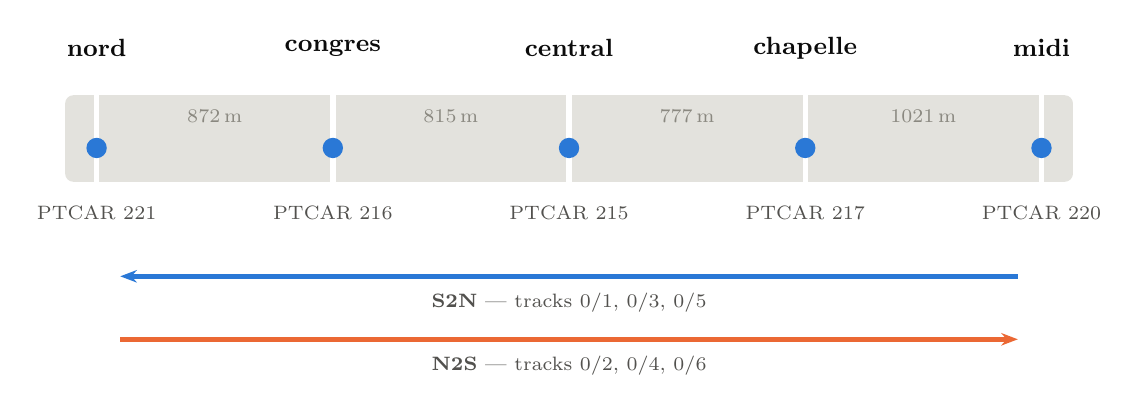
\begin{tikzpicture}[font=\small]
    % tunnel band
    \fill[cgrid, rounded corners=3pt] (-0.4,-0.55) rectangle (12.4,0.55);
    % inter-station distances, inside the band
    \foreach \a/\b/\d in {0/3/872, 3/6/815, 6/9/777, 9/12/1021}{
      \pgfmathsetmacro\mid{(\a+\b)/2}
      \node[font=\scriptsize, color=ink3] at (\mid,0.28) {\d\,m};
    }
    \foreach \x/\nm/\pt in {0/nord/221, 3/congres/216, 6/central/215, 9/chapelle/217, 12/midi/220}{
      \draw[white, line width=2pt] (\x,-0.55) -- (\x,0.55);
      \node[circle, fill=cblue, inner sep=2.6pt] at (\x,-0.12) {};
      \node[font=\small\bfseries, color=ink] at (\x,1.15) {\nm};
      \node[font=\scriptsize, color=ink2] at (\x,-0.95) {PTCAR \pt};
    }
    % direction arrows, well clear of the PTCAR row
    \draw[-{Stealth[length=6pt]}, cblue, line width=1.6pt] (11.7,-1.75) -- (0.3,-1.75);
    \node[font=\scriptsize, color=ink2] at (6,-2.08) {\textbf{S2N} --- tracks 0/1, 0/3, 0/5};
    \draw[-{Stealth[length=6pt]}, corange, line width=1.6pt] (0.3,-2.55) -- (11.7,-2.55);
    \node[font=\scriptsize, color=ink2] at (6,-2.88) {\textbf{N2S} --- tracks 0/2, 0/4, 0/6};
  \end{tikzpicture}}

  \vspace{0.6em}
  \raggedright
  \begin{columns}[T]
    \begin{column}{0.48\textwidth}\small
      $\approx$3.5\,km end to end $\cdot$ hops of 777--1021\,m\\
      \textbf{968 traversals per day}, both directions
    \end{column}
    \begin{column}{0.48\textwidth}\small
      Six tracks, \textbf{three per direction}, each strictly one-directional\\
      A train holds \emph{one} track for the whole crossing
    \end{column}
  \end{columns}
\end{frame}

\begin{frame}{Identifying the junction}
  \texttt{PTCAR\_NO} uses the same numbering as \texttt{STATIONS} in
  \texttt{core/simulation/build\_hard.py}, confirmed against the Infrabel reference
  dataset \texttt{operationele-punten-van-het-netwerk} (1{,}359 points with coordinates).

  \vspace{0.8em}
  \centering
  \begin{tabular}{@{}rlllr@{}}
    \toprule
    PTCAR & Symbolic & Name (FR) & Data name (NL) & lat, lon \\
    \midrule
    215 & FBCL & BRUXELLES-CENTRAL & BRUSSEL-CENTRAAL & 50.845, 4.357 \\
    216 & FBCO & BRUXELLES-CONGRES & BRUSSEL-CONGRES & 50.852, 4.362 \\
    217 & FBCK & BRUXELLES-CHAPELLE & BRUSSEL-KAPELLEKERK & 50.841, 4.348 \\
    220 & FBMZ & BRUXELLES-MIDI & BRUSSEL-ZUID & 50.836, 4.336 \\
    221 & FBN & BRUXELLES-NORD & BRUSSEL-NOORD & 50.860, 4.361 \\
    \bottomrule
  \end{tabular}

  \vspace{1em}
  \raggedright
  \srcnote{216 and 217 are classified \emph{stop in open track}, not stations --- they are
  95--98\% pass-through in the data, which matters later.}
\end{frame}

\begin{frame}{Transformation pipeline --- exactly what was done}
  \centering
  \resizebox{\textwidth}{!}{%
  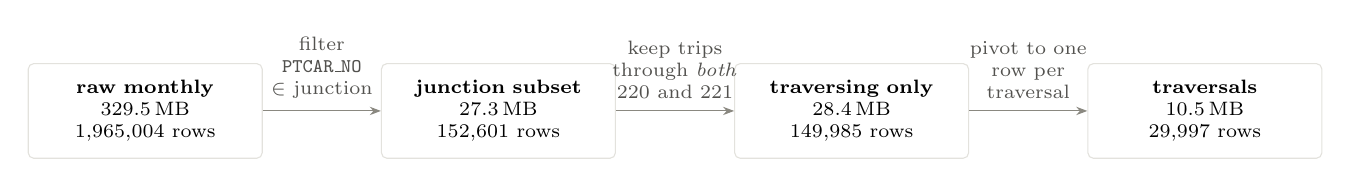
\begin{tikzpicture}[
      node distance=0.55cm,
      box/.style={draw=cgrid, fill=white, rounded corners=2pt, align=center,
                  inner sep=6pt, font=\scriptsize, text width=2.55cm},
      lbl/.style={font=\scriptsize\color{ink2}, align=center, text width=2.6cm},
      arr/.style={-{Stealth[length=4pt]}, draw=ink3}]
    \node[box] (raw) {\textbf{raw monthly}\\329.5\,MB\\1{,}965{,}004 rows};
    \node[box, right=1.5cm of raw] (junc) {\textbf{junction subset}\\27.3\,MB\\152{,}601 rows};
    \node[box, right=1.5cm of junc] (trav) {\textbf{traversing only}\\28.4\,MB\\149{,}985 rows};
    \node[box, right=1.5cm of trav] (wide) {\textbf{traversals}\\10.5\,MB\\29{,}997 rows};

    \draw[arr] (raw) -- node[lbl, above=1pt] {filter\\\texttt{PTCAR\_NO}\\$\in$ junction} (junc);
    \draw[arr] (junc) -- node[lbl, above=1pt] {keep trips\\through \emph{both}\\220 and 221} (trav);
    \draw[arr] (trav) -- node[lbl, above=1pt] {pivot to one\\row per\\traversal} (wide);
  \end{tikzpicture}}

  \vspace{1.2em}
  \raggedright
  \begin{itemize}\small
    \item \textbf{Step 1} \texttt{extract\_junction.py} --- streams the raw file once
      ($\approx$7\,s), keeps the 5 junction PTCARs. Retains 7.77\% of rows.
    \item \textbf{Step 2} keep only trains passing through \emph{both} Nord and Midi, i.e.
      that actually traverse. Drops 2{,}616 single-station touches (2{,}532 at Midi).
    \item \textbf{Step 3} \texttt{build\_traversals.py} --- pivot the 5 points into
      \texttt{p1..p5} \hl{ordered along direction of travel}, add \texttt{direction},
      \texttt{tunnel\_track}, \texttt{entry\_delay}, \texttt{exit\_delay},
      \texttt{delay\_gained}.
  \end{itemize}
\end{frame}

\begin{frame}{Reading a traversal row --- what \texttt{p1}\dots\texttt{p5} mean}
  After the pivot, each row is \emph{one train crossing the junction once}, and the five
  measurement points become columns \texttt{p1\_*} through \texttt{p5\_*}.

  \vspace{0.4em}
  \begin{alertblock}{\small \texttt{p1}\dots\texttt{p5} are positions \emph{along travel}, not fixed stations}
    \small \texttt{p1} is always the point the train \textbf{enters} at and \texttt{p5} the
    point it \textbf{leaves} at --- so \texttt{p1} is Nord for an N2S train but Midi for an
    S2N train. This is deliberate: it makes
    \texttt{p1\_delay\_arr}\,\dots\,\texttt{p5\_delay\_arr} a single comparable sequence
    ``entry $\to$ exit'' regardless of direction.
  \end{alertblock}

  \vspace{0.3em}
  \centering\scriptsize
  \texttt{train\_no=1945 $\cdot$ IC 06-1: BRUSSELS AIRPORT $\to$ TOURNAI $\cdot$
  direction=N2S $\cdot$ tunnel\_track=0/4}

  \vspace{0.3em}
  \begin{tabular}{@{}llrrrrl@{}}
    \toprule
    & point & arrival & \texttt{delay\_arr} & departure & \texttt{delay\_dep} & \texttt{stop\_type} \\
    \midrule
    \texttt{p1} & nord (221) & 23:58:50 & $-9$ & 0:01:11 & $+11$ & \texttt{=} stop \\
    \texttt{p2} & congres (216) & 0:03:15 & $+15$ & 0:03:15 & $+15$ & \texttt{D} pass-through \\
    \texttt{p3} & central (215) & 0:04:50 & $-9$ & 0:06:16 & $+16$ & \texttt{=} stop \\
    \texttt{p4} & chapelle (217) & 0:07:20 & $-40$ & 0:07:20 & $-40$ & \texttt{D} pass-through \\
    \texttt{p5} & midi (220) & 0:09:25 & $-34$ & \color{corange}\textit{(blank)} & \color{corange}\textit{(blank)} & \color{corange}\textit{(blank)} \\
    \bottomrule
  \end{tabular}

  \vspace{0.5em}
  \raggedright\small
  \texttt{entry\_delay} $=$ \texttt{p1\_delay\_dep} $= +11$\,s \quad
  \texttt{exit\_delay} $=$ \texttt{p5\_delay\_arr} $= -34$\,s \quad
  \hl{\texttt{delay\_gained} $= -45$\,s}

  \srcnote{Note this row also crosses midnight (23:58 $\to$ 00:09) while \texttt{date} stays
  on 01JAN --- one of 59 such traversals. And it shows the blank pattern explained next.}
\end{frame}

\begin{frame}{Structural facts that shaped everything downstream}
  \begin{columns}[T]
    \begin{column}{0.5\textwidth}
      \textbf{The structure is completely regular}
      \begin{itemize}\small
        \item 29{,}997 of 32{,}613 trips give \emph{exactly} 5 rows
        \item Zero fell into ``unexpected order'' or ``not five points''
        \item Only two row orders occur, evenly split:
          $220\!\to\!217\!\to\!215\!\to\!216\!\to\!221$ (S2N, 14{,}964) and its
          reverse (N2S, 15{,}033)
        \item \hl{Direction is recoverable from row order alone}
      \end{itemize}
      \vspace{0.6em}
      \textbf{Tunnel tracks are one-directional}\\[0.3em]
      \srcnote{Each traversal holds a \emph{single} tunnel track across
      215/216/217 --- verified: distinct-track-count per trip is 1 in all 29{,}997 cases.}
    \end{column}
    \begin{column}{0.48\textwidth}
      \centering\small
      \begin{tabular}{@{}llr@{}}
        \toprule
        Track & Direction & Traversals \\
        \midrule
        0/1 & S2N & 5{,}673 \\
        0/2 & N2S & 5{,}890 \\
        0/3 & S2N & 5{,}502 \\
        0/4 & N2S & 5{,}767 \\
        0/5 & S2N & 3{,}789 \\
        0/6 & N2S & 3{,}376 \\
        \bottomrule
      \end{tabular}
      \vspace{1em}

      \raggedright\srcnote{Odd tracks southbound-to-north, even tracks
      north-to-south. Three per direction --- the six-track N--S tunnel.}
    \end{column}
  \end{columns}
\end{frame}

\begin{frame}{What a ``blank'' is, and where they occur}
  \textbf{A blank is simply an empty cell} in the CSV --- Infrabel recorded no value for
  that field on that row. Each measurement point has \emph{two} sides, an arrival and a
  departure, and either can be blank independently.

  \vspace{0.7em}
  Across the 29{,}997 traversals, blanks appear at \textbf{exactly two of the ten
  delay columns}:

  \vspace{0.4em}
  \centering
  \begin{tabular}{@{}llrl@{}}
    \toprule
    Column & Side & Blank rows & \\
    \midrule
    \texttt{p1\_delay\_arr} & arrival at the \textbf{entry} point & 4{,}741 & \\
    \texttt{p5\_delay\_dep} & departure at the \textbf{exit} point & 4{,}789 & \\
    \addlinespace
    \texttt{p1\_delay\_dep}, \texttt{p2..p4}, \texttt{p5\_delay\_arr}
      & (all others) & \textbf{0} & \color{caqua}\textbf{never blank} \\
    \bottomrule
  \end{tabular}

  \vspace{0.9em}
  \raggedright
  They come as a \textbf{bundle}: on a \texttt{p5}-blank row, \texttt{THOP1\_COD},
  \texttt{PLANNED\_TIME\_DEP}, \texttt{REAL\_TIME\_DEP} and \texttt{LINE\_NO\_DEP} are
  \emph{all} empty together (4{,}701 of 4{,}720) while the arrival fields are fully
  populated. So it is one coherent ``no onward record at this point'' class, heavily
  concentrated at Midi (4{,}336 of 4{,}720).
\end{frame}

\begin{frame}{Why the blanks do not hurt us --- and what we must not claim}
  \begin{block}{\small The convenient part}
    \small \texttt{delay\_gained} $=$ \texttt{p5\_delay\_arr} $-$ \texttt{p1\_delay\_dep}
    --- the arrival at the exit minus the departure at the entry. Those are precisely the
    two sides that are \textbf{never blank}. \hl{So \texttt{delay\_gained} is present for
    all 29{,}997 traversals}: no imputation, no row-dropping, for the headline propagation
    variable.
  \end{block}

  \vspace{0.6em}
  \begin{alertblock}{\small The tempting-but-wrong explanation}
    \small It looks like ``the train terminated there, so there is no departure.''
    \textbf{That reading does not survive checking:}
    \begin{itemize}\small
      \item Some of these trains \emph{do} end at Brussel-Zuid
        (\texttt{IC 35: ROTTERDAM CENTRAAL -> BRUSSEL-ZUID}).
      \item But others plainly continue --- our worked example
        \texttt{IC 06-1 -> TOURNAI}, and \texttt{IC 29: DE PANNE -> LEUVEN}.
      \item And the feed \emph{has} an origin/terminus code, \texttt{THOP1\_COD = P} ---
        \textbf{no Midi row ever carries it}.
    \end{itemize}
  \end{alertblock}

  \vspace{0.4em}
  \centering
  Treat it as a \textbf{recording gap of unconfirmed cause}. Worth asking Infrabel.
\end{frame}

% =============================================================== PART II
\section{Part II --- State of the art}
\begin{frame}[plain]
  \begin{center}\Large\textbf{Part II --- State of the art}\end{center}
\end{frame}

\begin{frame}{Three predictive paradigms}
  \begin{enumerate}
    \item \textbf{Spatio-temporal GNNs.} Heterogeneous graphs (SAGE-Het) with train,
      station and time-slot node types; graph attention (GATv2) to weight propagation
      dynamically. \srcnote{Li et al.\ 2024; Nguyen \& Li 2025.}
    \item \textbf{Simulation-driven imitation learning.} Reframes forecasting as stochastic
      simulation of state transitions; DCIL extends DAgger with drift correction to fight
      covariate shift in rollouts. \srcnote{Elliker et al.\ 2025 --- \emph{on Infrabel data}.}
    \item \textbf{Tree ensembles + conformal prediction.} GBDTs on tabular history, paired
      with distribution-free prediction intervals for dispatching support.
  \end{enumerate}

  \vspace{1em}
  \begin{block}{\small The benchmark that matters for us}
    \small \textbf{RIDE} (arXiv 2606.05070) --- open benchmark on the \hl{Belgian} network:
    94.5M train events, 3.6M journeys, \hl{35.7M weather records}, 2023--2025, keyed to
    operational points. Weather is our largest missing input and RIDE is aligned to our
    identifiers.
  \end{block}
\end{frame}

\begin{frame}{Causal discovery and causal ML}
  \begin{itemize}
    \item \textbf{Reconstructing the propagation network.} Constraint-based discovery
      (PC/FCI) and PCMCI on lagged multivariate series; Hawkes--Granger processes for
      event-triggered propagation.
    \item \textbf{``What-if'' dispatching.} Framing a hold-or-not decision as a treatment
      and estimating ITE/ATE, to separate deliberate dispatcher action from natural
      propagation.
    \item \textbf{Unified GNN + CML + conformal} frameworks.
  \end{itemize}

  \vspace{0.8em}
  \begin{alertblock}{\small Verification matters --- claims checked individually}
    \small
    \begin{itemize}\small
      \item \textbf{``GNNs consistently achieve the lowest MAE'' is inverted} for the paper
        it rests on: Nguyen \& Li report \emph{``the much simpler Persistence baseline
        achieves the best scores on MAE and RMSE.''} Their GATv2 wins on \emph{precision}.
      \item \textbf{PCMCI-on-railway} and \textbf{conformal-prediction-on-train-delay}:
        no arXiv evidence found. Good ideas, not established practice.
      \item A \textbf{Scientific Reports ``unified GNN+CML+CP'' paper} turns out not to be a
        delay paper at all: target is \emph{total Vehicle\,KM}, $n=288$ line-level
        aggregates, and the word ``delay'' appears 5 times, all in related work.
    \end{itemize}
  \end{alertblock}
\end{frame}

\begin{frame}{What actually applies at our scale}
  Our unit is a \textbf{5-node, 6-track junction}, one month, 29{,}997 traversals.

  \vspace{0.8em}
  \centering
  \begin{tabular}{@{}p{4.1cm}p{8.3cm}@{}}
    \toprule
    \textbf{Do now} & Persistence baseline; conformal intervals (heavy tails);
      GBDT on the tabular traversal table \\
    \addlinespace
    \textbf{Tested, adds nothing} & Weather at junction scale: $-1.7\%$ MAE, six features
      (Step 7). RIDE's 2023--2025 span is the way to test it properly \\
    \addlinespace
    \textbf{Overkill} & ST-GNN on 5 nodes --- no topology to learn. Same objection applies to
      Dekker's diffusion model \\
    \addlinespace
    \textbf{Blocked} & Causal ML for dispatching --- needs intervention logs that the
      Infrabel feed does not contain \\
    \bottomrule
  \end{tabular}

  \vspace{1.2em}
  \raggedright
  \srcnote{One convergence worth noting: Nguyen's explainability analysis finds the model
  keys on local congestion to spot fragile states where \emph{inter-train headway conflicts}
  propagate delay --- the same mechanism as Li's 20-minute threshold, and the same one we
  measure directly in Phase 0.}
\end{frame}

% =============================================================== PART III
\section{Part III --- Phase 0}
\begin{frame}[plain]
  \begin{center}\Large\textbf{Part III --- Phase 0}\end{center}
  \begin{center}\color{ink2}Observational facts, and a floor to beat\end{center}
\end{frame}

\begin{frame}{Phase 0 --- the steps}
  \begin{enumerate}
    \item Build the \textbf{leader/follower pair table} on shared tunnel track
    \item Define the \textbf{prediction task} and a temporal split
    \item \textbf{Baselines}: zero, persistence, mean-gain
    \item A \textbf{feature model} that must beat them
    \item Test \textbf{Dekker's exponential-decay claim}
    \item Facts sheet and figures
    \item Add \textbf{weather} and test whether it earns its place
  \end{enumerate}

  \vspace{1em}
  \begin{block}{\small In one sentence}
    \small Given how late a train is \textbf{entering} the junction, plus who is ahead of it
    and how close, predict how late it will be \textbf{leaving}. Next slide makes this precise.
  \end{block}
\end{frame}

\begin{frame}{The prediction task, precisely}
  \textbf{One row $=$ one train crossing the junction, paired with the train ahead of it on
  the same tunnel track.}

  \vspace{0.5em}
  \begin{columns}[T]
    \begin{column}{0.47\textwidth}
      \textbf{Output} \quad\srcnote{(continuous, signed seconds)}\\[0.25em]
      \texttt{follower\_exit\_delay} $=$ \texttt{p5\_delay\_arr}\\
      \srcnote{the train's delay on \emph{arrival} at the far side}

      \vspace{0.8em}
      \textbf{Prediction moment}\\[0.25em]
      the instant it \emph{departs} the entry point \texttt{p1}.\\
      \hl{Every feature must be known then.}

      \vspace{0.8em}
      \textbf{Baselines} predict the same target with no model:\\[0.2em]
      \srcnote{\texttt{zero}: 0 \quad$\cdot$\quad
      \texttt{persistence}: \texttt{entry\_delay} (the junction changes nothing)
      \quad$\cdot$\quad \texttt{mean-gain}: \texttt{entry\_delay} $+\,26.9$\,s}
    \end{column}
    \begin{column}{0.51\textwidth}
      \textbf{Input} --- seven features\\[0.3em]
      \small
      \begin{tabular}{@{}ll@{}}
        \toprule
        \texttt{entry\_delay} & its own delay leaving \texttt{p1} \\
        \texttt{hour} & hour of entry \\
        \texttt{tunnel\_track} & which of the six tracks \\
        \texttt{direction} & N2S or S2N \\
        \texttt{service} & IC / L / P / EURST \\
        \midrule
        \multicolumn{2}{@{}l@{}}{\color{corange}\textbf{interaction block}} \\
        \texttt{headway\_s} & gap to the train ahead \\
        \texttt{leader\_entry\_delay} & its delay when \emph{it} entered \\
        \bottomrule
      \end{tabular}
    \end{column}
  \end{columns}

  \vspace{0.7em}
  \srcnote{\textbf{Unit of observation:} the \emph{pairs} table, not the traversals table. A
  pair needs a predecessor, so the first traversal of each
  \texttt{(date, direction, track)} group has none --- 29{,}997 $\to$ \textbf{29{,}685 rows},
  312 dropped. \quad \textbf{Split:} temporal, train days 1--24 (22{,}817), test days 25--31
  (6{,}868); no shuffling. No distribution shift (means 163.4 vs 159.5\,s, p90 406 both).}
\end{frame}

\begin{frame}{Step 1 --- pairs, and a leakage trap}
  A \emph{pair} is two consecutive traversals sharing
  \texttt{(date, direction, tunnel\_track)}. \textbf{29{,}685 pairs}, median headway
  \textbf{5.3 min}. \srcnote{(312 traversals have no predecessor in their group and drop out.)}

  \vspace{0.8em}
  \begin{alertblock}{\small The trap}
    \small Median headway (5.3\,min) is \emph{shorter} than median traversal time
    (8.8\,min), so \textbf{the leader is usually still inside the junction} when the
    follower enters. \texttt{leader\_exit\_delay} is therefore \hl{not knowable at
    prediction time}. Models use \texttt{leader\_entry\_delay} instead.
  \end{alertblock}

  \vspace{0.5em}
  This costs most of the apparent signal --- and that is the honest picture:

  \centering\small
  \begin{tabular}{@{}lrr@{}}
    \toprule
    Headway & $r$(leader \textbf{exit}, follower gain) & $r$(leader \textbf{entry}, follower gain) \\
    \midrule
    $<$5 min & 0.275 & \textbf{0.119} \\
    5--10 min & 0.106 & 0.015 \\
    10--20 min & 0.046 & 0.023 \\
    20--60 min & 0.088 & 0.073 \\
    \bottomrule
  \end{tabular}
\end{frame}

\begin{frame}{Step 1 --- knock-on decays with headway}
  \centering
  \includegraphics[width=0.82\textwidth]{fig2_headway_knockon}

  \vspace{0.4em}
  \raggedright\srcnote{Coupling decays monotonically and is essentially gone by 10--20
  minutes --- independently reproducing Li et al.'s $\approx$20-minute interaction horizon on
  Brussels data. The junction operates deep inside the interacting regime: 96\% of
  consecutive same-track pairs are under 20 minutes.}
\end{frame}

\begin{frame}{Steps 2--4 --- baselines and the feature model}
  \centering
  \begin{tabular}{@{}lrrrr@{}}
    \toprule
    & \multicolumn{2}{c}{\textbf{regression}} & \multicolumn{2}{c}{\color{ink3}\emph{derived}: $>$300\,s event} \\
    \cmidrule(lr){2-3}\cmidrule(lr){4-5}
    Model & MAE (s) & RMSE (s) & Precision & Recall \\
    \midrule
    zero & 171.4 & 380.3 & --- & 0.000 \\
    \textbf{persistence} & \textbf{60.2} & \textbf{99.4} & 0.960 & 0.653 \\
    mean-gain & 63.1 & 94.1 & 0.919 & 0.694 \\
    GBDT (no interaction) & 66.1 & 143.2 & 0.931 & 0.698 \\
    \textbf{GBDT (+ headway/leader)} & \textbf{57.4} & 127.1 & 0.937 & 0.710 \\
    \bottomrule
  \end{tabular}

  \vspace{1em}
  \raggedright
  \begin{enumerate}\small
    \item \textbf{Persistence is hard to beat.} A GBDT with entry delay, hour, track,
      direction and service but \emph{no interaction features} \hl{loses to it by 9.7\%}.
    \item \textbf{Only the headway/leader block beats the baseline} --- worth $+8.63$\,s MAE
      (13.1\%), the entire source of the win. \emph{The one feature block with a causal story
      is the one carrying signal.}
    \item Margin is stable under rolling origin ($+6.1\%$, $+4.6\%$) --- not a one-week fluke.
  \end{enumerate}

  \vspace{0.3em}
  \srcnote{Precision/recall above are \emph{not} a second model --- see next slide.}
\end{frame}

\begin{frame}{On the ``$>$5 minutes late'' event --- we are not doing classification}
  \textbf{Every model in Phase 0 is a regressor.} The precision and recall columns are the
  \emph{regression output thresholded post-hoc} at 300\,s
  (\texttt{common.py:scores()}: \texttt{y\_pred > threshold}). There is no classifier.

  \vspace{0.5em}
  \textbf{Why report it.} The operational question is not ``how many seconds'' but ``will this
  train be more than 5 minutes late'' --- and it is the metric on which Nguyen \& Li's GATv2
  wins while \emph{losing} on MAE.

  \vspace{0.5em}
  \textbf{Why it is under-served.} A squared-error regressor does not optimise that event:

  \vspace{0.2em}
  \centering\small
  \begin{tabular}{@{}lrrr@{}}
    \toprule
    Approach & Precision & Recall & F1 \\
    \midrule
    persistence, thresholded & \textbf{0.960} & 0.653 & 0.777 \\
    GBDT regressor, thresholded \srcnote{(reported above)} & 0.937 & 0.710 & 0.807 \\
    \textbf{GBDT classifier trained on the event} & 0.935 & \textbf{0.743} & \textbf{0.828} \\
    \bottomrule
  \end{tabular}

  \vspace{0.4em}
  \raggedright\small
  Same precision, \hl{$+3.3$ points of recall}, and the threshold becomes a tunable knob
  rather than an artifact of the loss. \srcnote{Base rate in test: 14.8\%.}

  \vspace{0.3em}
  \textbf{Recommendation.} Keep regression primary --- \texttt{delay\_gained} is the causal
  quantity SUMO must reproduce --- but if the 5-minute event drives dispatching,
  \textbf{train for it explicitly}.
\end{frame}

\begin{frame}{Where the model breaks --- and why}
  \centering
  \includegraphics[width=0.78\textwidth]{fig3_rmse_by_headway}

  \vspace{0.3em}
  \raggedright\small
  The global RMSE loss (127.1 vs 99.4) is \emph{not} a tail problem. It localises entirely to
  the $>$20\,min band --- 3.7\% of training rows --- where the model extrapolates badly.
  \hl{The fix comes from Li et al.\ 2024}: above $\approx$20\,min there \emph{is} no train
  interaction, so those features are noise. Gating to persistence above the threshold gives
  \textbf{56.0 MAE / 92.4 RMSE}, beating persistence on both.

  \srcnote{Caveat: gating repairs the second fold, not the first. RMSE remains partly
  unexplained --- MAE gain is established, the RMSE story is not yet closed.}
\end{frame}

\begin{frame}{Step 5 --- testing Dekker's exponential decay}
  \textbf{Claim.} A station sheds delay in proportion to the delay it carries,
  $\mathrm{d}D/\mathrm{d}t = -B_i D_i$ --- so the change in a train's delay should be
  \emph{linear} in delay carried, with \emph{negative} slope.

  \vspace{0.6em}
  \textbf{Method.} Per direction and segment, regress change-in-delay on delay-carried.
  Dwell rows restricted to trains that actually stop (\texttt{stop\_type = '='}) ---
  \hl{Congr\`es and Chapelle are 95--98\% pass-through}, where
  \texttt{arr}\,$=$\,\texttt{dep} by construction and the regression would be
  definitionally zero.

  \vspace{0.8em}
  \begin{center}
    \textbf{4 of 17 segments consistent \quad$\cdot$\quad 0 contradict \quad$\cdot$\quad 13 flat}
  \end{center}

  \vspace{0.5em}
  \begin{itemize}\small
    \item \textbf{Consistent} --- dwell at the two terminals only: Midi ($-0.058$ S2N,
      $-0.034$ N2S), Nord ($-0.070$ S2N, $-0.052$ N2S).
    \item \textbf{Flat} --- dwell at Central, and \emph{every} run segment
      ($|\text{slope}|\le 0.019$), but with nonzero intercepts ($+6.2$, $+8.8$, $-17.1$,
      $-25.3$\,s).
  \end{itemize}
\end{frame}

\begin{frame}{Step 5 --- additive, not multiplicative}
  \centering
  \includegraphics[width=0.74\textwidth]{fig4_dekker_decay}

  \vspace{0.3em}
  \raggedright\small
  Between points, delay changes by a roughly \textbf{constant offset independent of the delay
  carried}. The diffusion model's core mechanism does \emph{not} operate at junction scale,
  except at the two big terminals where long dwells give room to recover proportionally.

  \srcnote{A useful negative result: a proportional-decay term is the wrong functional form
  here. The right skeleton is a constant per-segment offset plus a terminal recovery term ---
  and that is a concrete calibration target for SUMO.}
\end{frame}

\begin{frame}{The propagation profile}
  \centering
  \includegraphics[width=0.92\textwidth]{fig1_delay_profile}

  \vspace{0.3em}
  \raggedright\small
  Delay accumulates monotonically through the tunnel, then \emph{drops} on the last hop
  (congr\`es 81 $\to$ nord 74; chapelle 60 $\to$ midi 47). Nothing physical removes delay
  there --- it is \hl{recovery margin padded into the final approach}.

  \srcnote{Consequence: the p4$\to$p5 hop must be excluded from any propagation fit, or
  modelled separately and labelled. Otherwise it reads as ``the junction heals delay''.}
\end{frame}

\begin{frame}{Why point forecasts are not enough}
  \centering
  \includegraphics[width=0.72\textwidth]{fig5_delay_tail}

  \vspace{0.3em}
  \raggedright\small
  Mean 162\,s against median 61\,s; p99 at 1658\,s. Delay gained across the junction has
  median $\approx 0$ but mean $\approx +28$\,s --- the junction is neutral for a typical
  train and the average is driven entirely by a heavy right tail.

  \vspace{0.4em}
  \hl{Any model fit on the mean is fitting the tail.} This is the concrete argument for
  \textbf{conformal prediction intervals} rather than point estimates.
\end{frame}

\begin{frame}{Step 7 --- weather (a negative result)}
  \textbf{Method.} Replicated RIDE's own recipe (arXiv 2606.05070): Open-Meteo Historical
  Weather API, queried per operational point, timezone \texttt{Europe/Brussels}, six hourly
  variables --- \texttt{temperature\_2m}, \texttt{rain}, \texttt{snowfall},
  \texttt{relative\_humidity\_2m}, \texttt{wind\_speed\_10m}, \texttt{weather\_code} ---
  attached at the \hl{entry point and entry hour}, i.e.\ the prediction moment.
  100\% join rate.

  \vspace{0.4em}
  \srcnote{January 2025 was not a quiet month: mean 2.8\,$^\circ$C, 200 sub-zero hours,
  174 rain hours, 38 snowfall hours.}

  \vspace{0.4em}
  \centering\small
  \begin{tabular}{@{}lrr@{}}
    \toprule
    Model & MAE (s) & RMSE (s) \\
    \midrule
    persistence & 60.2 & 99.4 \\
    \textbf{GBDT (+ headway/leader)} & \textbf{57.4} & 127.1 \\
    GBDT (+ weather) & 58.4 & 129.7 \\
    \bottomrule
  \end{tabular}

  \vspace{0.5em}
  \raggedright\small
  The weather block is worth $-0.99$\,s MAE ($-1.7\%$) --- six added features, and
  \hl{slightly worse}. No help in the bad-weather subgroup either (rain $>$0.5\,mm, snowfall,
  or sub-zero; $n=855$): 49.2\,s MAE with weather against \textbf{48.0} without.

  \vspace{0.5em}
  \textbf{And this is the expected answer.} The junction is a 3.5\,km sheltered tunnel and a
  train is inside for $\approx$9 minutes. Weather acts on the \emph{network}; its effect
  arrives already encoded in \texttt{entry\_delay}, the model's first feature.
\end{frame}

\begin{frame}{Step 7 --- weather is not the confounder}
  \begin{block}{\small The result that matters}
    \small Weather was the most plausible latent common cause behind the leader/follower
    correlation --- and it is not it. Partial correlation of
    \texttt{leader\_entry\_delay} vs \texttt{follower\_delay\_gained}, headway $<$5 min:
    \vspace{0.3em}
    \begin{center}
    \begin{tabular}{@{}lr@{}}
      \toprule
      raw \srcnote{(the 0.119 of Step 1)} & $+0.1195$ \\
      controlling for weather & $+0.1217$ \\
      controlling for weather $+$ hour & $+0.1151$ \\
      \bottomrule
    \end{tabular}
    \end{center}
    \vspace{0.2em}
    \hl{Essentially unchanged} --- which strengthens the case that the coupling is a genuine
    track-occupancy mechanism rather than shared exposure.
  \end{block}

  \vspace{0.5em}
  \begin{alertblock}{\small The one apparent signal was a single day}
    \small Daily snowfall against mean entry delay gives $r = +0.414$
    (95\% CI $[+0.07, +0.67]$, $n=31$) --- but dropping 09JAN2025, the one heavy snow day,
    collapses it to $r = -0.007$. Snow days average 138\,s entry delay against 132\,s on
    dry days.
  \end{alertblock}

  \vspace{0.3em}
  \srcnote{This says weather adds nothing to \emph{this} model at \emph{this} scale, not that
  weather is irrelevant to Belgian rail delay. One month, six snow days, one that matters.
  Testing it properly needs RIDE's 2023--2025 span.}
\end{frame}

\begin{frame}{Phase 0 --- conclusions}
  \begin{enumerate}
    \item \textbf{A floor exists and it is high.} Persistence: MAE 60.2, RMSE 99.4. Feature
      richness alone does not beat it.
    \item \textbf{The causal feature block is the only one that pays.} Headway + leader state
      is the entire margin --- arrived at empirically, not assumed.
    \item \textbf{Knock-on is real, concentrated, and short-range.} Strongest below 5\,min,
      gone by 10--20\,min, matching the literature. But most of the apparent signal is
      post-hoc and unusable in advance.
    \item \textbf{Dekker's proportional shedding is mostly falsified} at junction scale.
      Delay change is additive between points; proportional only at terminals.
    \item \textbf{Heavy tails demand intervals}, not point estimates.
    \item \textbf{Weather adds nothing at junction scale} --- and, more usefully, is ruled out
      as the confounder behind the knock-on correlation.
  \end{enumerate}
\end{frame}

\begin{frame}{Step 9 --- the full year: what survives}
  All 12 months of 2025 fetched: \textbf{338{,}914 traversals}, 335{,}323 pairs.
  \srcnote{(Three months first arrived truncated --- a 342\,MB file returned as 1\,MB,
  ending the read cleanly with no error. The fetcher now verifies \texttt{Content-Length}.)}

  \vspace{0.5em}
  \begin{alertblock}{\small January was the best month of the year}
    \small \texttt{delay\_gained} median \textbf{3\,s} in January against 12--13\,s in the
    worst months; mean 27.9\,s against 48.3\,s in October. The Phase 0 headline numbers are
    correct but \emph{not representative}.
  \end{alertblock}

  \vspace{0.4em}
  \centering
  \begin{tabular}{@{}lll@{}}
    \toprule
    & January said & Full year says \\
    \midrule
    Knock-on correlation & $+0.119$ &
      \textbf{survives}: mean $+0.110$, sd $0.018$, range $[+0.086, +0.148]$ \\
    Model beats persistence & $+6.1\%$, $+4.6\%$ &
      \textbf{downgraded}: $+4.0\%$ mean, 8 of 9 folds, loses in July \\
    RMSE gap & ``partly unexplained'' &
      \textbf{systematic}: worse in \emph{all} 9 folds \\
    Weather & no gain (6 snow days) &
      \textbf{settled}: $-0.07$\,s MAE; $r=+0.088$, CI includes 0 \\
    \bottomrule
  \end{tabular}

  \vspace{0.6em}
  \raggedright\small
  The RMSE degradation is no longer a fold artifact. Likely driver:
  \hl{month-to-month non-stationarity} (\texttt{gain\_mean} swings 27--48\,s), which argues
  for time-varying estimation rather than one static fit.
\end{frame}

% =============================================================== PART IV
\section{Part IV --- Causality}
\begin{frame}[plain]
  \begin{center}\Large\textbf{Part IV --- Causality}\end{center}
  \begin{center}\color{ink2}From ``they move together'' to ``it makes it happen''\end{center}
\end{frame}

\begin{frame}{Three designs, not one algorithm}
  Phase 0 established an \emph{association}: $r\approx+0.11$, stable across 12 months,
  unmoved by weather, hour or month. That is not the claim we want.

  \vspace{0.7em}
  \begin{columns}[T]
    \begin{column}{0.32\textwidth}
      \textbf{A. Discovery}\\[0.3em]
      \srcnote{PC and FCI search for the graph by conditional-independence testing, with the
      temporal order supplied as background knowledge. FCI admits \emph{latent} confounders
      instead of inventing a direct edge for them.}
    \end{column}
    \begin{column}{0.32\textwidth}
      \textbf{B. Negative control}\\[0.3em]
      \srcnote{A design, not an algorithm. The two rival explanations predict
      \emph{opposite} patterns across headway --- so the data can tell them apart.}
    \end{column}
    \begin{column}{0.32\textwidth}
      \textbf{C. Instrumental variable}\\[0.3em]
      \srcnote{The timetable as a natural experiment: scheduled headway is fixed months
      ahead, so today's disruption cannot have caused it.}
    \end{column}
  \end{columns}

  \vspace{0.9em}
  \begin{block}{\small Two statistical hazards, handled explicitly}
    \small
    At $n=313{,}151$ \textbf{every independence test rejects} --- significance is
    uninformative, so discovery uses subsampling with stability selection and everything is
    reported as \emph{effect size}. And the delay tail breaks Gaussian partial correlations,
    so all continuous variables are \textbf{rank-transformed to normal scores}.
  \end{block}
\end{frame}

\begin{frame}{Design A --- discovery with temporal background knowledge}
  \begin{columns}[T]
    \begin{column}{0.42\textwidth}
      10 variables in \textbf{4 temporal tiers}; 29 arrows forbidden because they would point
      backwards in time.

      \vspace{0.5em}
      \centering
      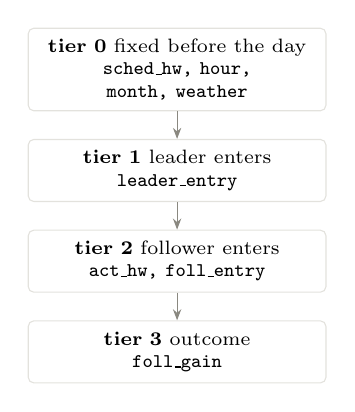
\begin{tikzpicture}[font=\scriptsize, node distance=0.35cm,
          t/.style={draw=cgrid, fill=white, rounded corners=2pt, inner sep=4pt,
                    text width=3.5cm, align=center}]
        \node[t] (t0) {\textbf{tier 0} fixed before the day\\
          \texttt{sched\_hw, hour, month, weather}};
        \node[t, below=of t0] (t1) {\textbf{tier 1} leader enters\\ \texttt{leader\_entry}};
        \node[t, below=of t1] (t2) {\textbf{tier 2} follower enters\\
          \texttt{act\_hw, foll\_entry}};
        \node[t, below=of t2] (t3) {\textbf{tier 3} outcome\\ \texttt{foll\_gain}};
        \draw[-{Stealth[length=4pt]}, ink3] (t0) -- (t1);
        \draw[-{Stealth[length=4pt]}, ink3] (t1) -- (t2);
        \draw[-{Stealth[length=4pt]}, ink3] (t2) -- (t3);
      \end{tikzpicture}
    \end{column}
    \begin{column}{0.56\textwidth}
      Edge retained in $\geq$50\% of 40 subsamples ($n=4{,}000$ each):

      \vspace{0.4em}
      \small
      \begin{tabular}{@{}lrr@{}}
        \toprule
        edge & PC & FCI \\
        \midrule
        \texttt{act\_hw} $\to$ \texttt{foll\_gain} & \textbf{100\%} & \textbf{100\%} \\
        \texttt{leader\_entry} $\to$ \texttt{act\_hw} & 100\% & 100\% \\
        \texttt{leader\_entry} $\to$ \texttt{foll\_entry} & 100\% & 100\% \\
        \texttt{sched\_hw} $\to$ \texttt{act\_hw} & 100\% & 100\% \\
        \midrule
        \texttt{leader\_entry} --- \texttt{foll\_gain} \srcnote{(direct)}
          & \hl{45\%} & \hl{22\%} \\
        \bottomrule
      \end{tabular}

      \vspace{0.7em}
      \textbf{Headway is a stable direct cause. The direct leader$\to$follower edge is not}
      --- and survives even less under FCI, i.e.\ once latent confounding is allowed for.

      \vspace{0.3em}
      Recovered route: \hl{\texttt{leader\_entry} $\to$ \texttt{act\_hw} $\to$ \texttt{foll\_gain}}
    \end{column}
  \end{columns}
\end{frame}

\begin{frame}{Design B --- the negative control}
  \begin{block}{\small Why this is the sharpest test observational data allows}
    \small The two explanations predict \textbf{opposite} things.
    A physical track-occupancy mechanism \emph{must} weaken as trains separate.
    Shared upstream disruption \emph{should not} --- a disruption hits near and far trains
    alike. So the data can discriminate.
  \end{block}

  \vspace{0.5em}
  \centering
  \begin{tabular}{@{}lrrr@{}}
    \toprule
    headway & $n$ & raw $r$ & partial $r$ \srcnote{(given hour, month, weather)} \\
    \midrule
    $<$3 min & 49{,}073 & \textbf{0.243} & 0.243 \\
    3--5 min & 87{,}944 & 0.189 & 0.189 \\
    5--10 min & 112{,}003 & 0.074 & 0.074 \\
    10--20 min & 50{,}954 & 0.026 & 0.026 \\
    20--40 min & 12{,}195 & 0.008 & 0.012 \\
    40--120 min & 982 & 0.005 & $-0.001$ \\
    \bottomrule
  \end{tabular}

  \vspace{0.7em}
  \raggedright
  \hl{Monotone decay to zero} --- the mechanism prediction, not the confounding one.
  And partial $\approx$ raw throughout: the confounders we can measure explain \emph{none}
  of it.
\end{frame}

\begin{frame}{Design C --- the timetable as a natural experiment}
  \textbf{Instrument.} Scheduled headway is set by a timetable fixed months in advance, so it
  cannot be caused by today's disruption --- yet it strongly drives actual headway.

  \vspace{0.5em}
  \centering
  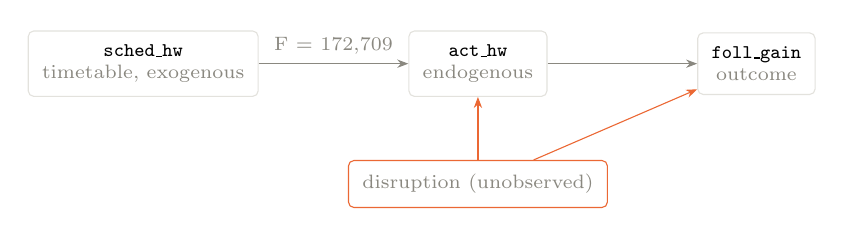
\begin{tikzpicture}[font=\scriptsize, node distance=1.5cm,
      b/.style={draw=cgrid, fill=white, rounded corners=2pt, inner sep=5pt, align=center}]
    \node[b] (z) {\texttt{sched\_hw}\\ \srcnote{timetable, exogenous}};
    \node[b, right=1.9cm of z] (x) {\texttt{act\_hw}\\ \srcnote{endogenous}};
    \node[b, right=1.9cm of x] (y) {\texttt{foll\_gain}\\ \srcnote{outcome}};
    \node[b, below=0.8cm of x, draw=corange] (u) {\srcnote{disruption (unobserved)}};
    \draw[-{Stealth[length=4pt]}, ink3] (z) -- node[above, font=\scriptsize]{F $=$ 172{,}709} (x);
    \draw[-{Stealth[length=4pt]}, ink3] (x) -- (y);
    \draw[-{Stealth[length=4pt]}, corange] (u) -- (x);
    \draw[-{Stealth[length=4pt]}, corange] (u) -- (y);
  \end{tikzpicture}

  \vspace{0.6em}
  \raggedright
  Controls: hour, month, track, direction. First stage
  $\mathrm{d}(\text{actual})/\mathrm{d}(\text{scheduled}) = +0.434$, partial $R^2 = 0.356$.

  \vspace{0.5em}
  \centering
  \begin{tabular}{@{}lr@{}}
    \toprule
    estimator & effect of $+1$ min headway on delay gained \\
    \midrule
    OLS & $-4.23$\,s \\
    \textbf{2SLS} & \hl{$-1.81$\,s} \quad bootstrap 95\% CI $[-2.06, -1.55]$ \\
    \bottomrule
  \end{tabular}

  \vspace{0.6em}
  \raggedright\small
  OLS overstates the magnitude by $\approx2.3\times$, in the expected direction: disruption
  both compresses headway \emph{and} raises delay, so the naive slope absorbs the
  confounding.
\end{frame}

\begin{frame}{How much goes through headway? --- and one failed test}
  \textbf{Mediation.} Headway $<$5 min, $n = 137{,}017$:

  \vspace{0.3em}
  \centering
  \begin{tabular}{@{}lr@{}}
    \toprule
    $r$(\texttt{leader\_entry}, \texttt{foll\_gain}) & $+0.2922$ \\
    \quad given context (hour, month, weather) & $+0.2925$ \\
    \quad given context $+$ \texttt{act\_hw} & $+0.1995$ \\
    \quad given context $+$ \texttt{act\_hw} $+$ \texttt{foll\_entry} & $+0.1496$ \\
    \bottomrule
  \end{tabular}

  \vspace{0.5em}
  \raggedright
  Headway removes about a third of the association. A residual $+0.15$ remains:
  \hl{partial, not complete, mediation} --- consistent with the unstable-but-nonzero direct
  edge in Design A.

  \vspace{0.7em}
  \begin{alertblock}{\small A test that failed, reported as failed}
    \small I tried a band-restricted IV as a falsification check, expecting $\approx0$ where
    no mechanism exists. It returned $-205$\,s/min at $<$5 min. \textbf{The design is
    invalid}: restricting to a headway band selects on the endogenous variable itself,
    collapsing the first stage and exploding the ratio. The near-zero value it gave at
    20--40 min is \emph{not} evidence of anything --- same broken setup. Only the
    full-sample IV estimate stands.
  \end{alertblock}
\end{frame}

\begin{frame}{What can be claimed --- and what cannot}
  \begin{enumerate}
    \item \textbf{Headway causally affects delay gained.} Stable under PC \emph{and} FCI,
      survives the negative control, quantified by a strong instrument:
      \hl{$\approx1.8$\,s per extra minute}.
    \item \textbf{The leader's delay acts mainly \emph{through} headway}, not directly ---
      though mediation is partial, with a residual direct association.
    \item \textbf{Measured confounders do not explain the coupling.} Weather, hour and month
      move the partial correlations essentially not at all.
  \end{enumerate}

  \vspace{0.8em}
  \begin{alertblock}{\small The limit of observational data}
    \small \textbf{Unmeasured confounding is not excluded.} FCI's reluctance to keep the
    direct edge is itself a hint that something latent sits behind it --- and no amount of
    conditioning on what we happen to have measured can settle that.

    \vspace{0.3em}
    This is exactly the gap the SUMO oracle closes: \hl{in simulation we \emph{set} headway
    rather than instrumenting it.} Design C approximates an experiment; Phase 2 runs one.
  \end{alertblock}
\end{frame}

% =============================================================== PART V
\section{Part V --- Reformulating the question}
\begin{frame}[plain]
  \begin{center}\Large\textbf{Part V --- Reformulating the question}\end{center}
  \begin{center}\color{ink2}The path matters as much as the answer\end{center}
\end{frame}

\begin{frame}{How we got here --- and where the reasoning broke}
  \begin{enumerate}
    \item \textbf{Starting assumption.} \emph{Delay propagates through the junction; model
      how.} The framing the whole literature uses --- Dekker's diffusion, Li's GNN,
      Nguyen's GAT. Never questioned.
    \item \textbf{The association.} \texttt{delay\_gained} median $\approx+7$\,s, mean
      $\approx+34$\,s, heavy tail. Summarised as \emph{``the junction is neutral for the
      typical train; the mean is a tail effect.''}
    \item \hl{The challenge.} \emph{``The hypothesis to test is whether the junction changes
      the delay at all --- and it doesn't seem to. Better to look at the cases where it did,
      and compare the distributions before and after.''}
  \end{enumerate}

  \vspace{0.8em}
  \begin{alertblock}{\small Step 2 was the weak link}
    \small It is arithmetically true and analytically misleading:
    \textbf{the median of the differences is not the difference of the medians.}
    We had been modelling \emph{how much} delay propagates without first establishing
    \emph{whether} the junction does anything.
  \end{alertblock}
\end{frame}

\begin{frame}{Testing it properly --- and a correction}
  \centering
  \includegraphics[width=0.93\textwidth]{fig6_dispersion}

  \vspace{0.2em}
  \raggedright\small
  \textbf{The junction does change delay.} Cohen's $d = 0.318$, KS $= 0.148$, and the median
  of the distribution moves $34 \to 63$\,s. But the mechanism is \hl{dispersion, not
  translation}: the 5th percentile moves \emph{down} ($-6 \to -37$\,s) while the 99th moves
  \emph{up} ($585 \to 730$\,s). Standard deviation $141 \to 184$\,s.

  \srcnote{Invisible if you look only at central tendency --- which is exactly what step 2 did.}
\end{frame}

\begin{frame}{The mass sits in a minority}
  \begin{columns}[T]
    \begin{column}{0.46\textwidth}
      \begin{tabular}{@{}lr@{}}
        \toprule
        $|$gain$| \leq 60$\,s & \textbf{71.3\%} \\
        gain $> +60$\,s & 24.8\% \\
        gain $< -60$\,s & 3.9\% \\
        \bottomrule
      \end{tabular}

      \vspace{0.8em}
      That \textbf{24.8\%} accounts for \hl{118\%} of all delay the junction adds.
      \srcnote{(Over 100\% because the 3.9\% recovering more than a minute offsets it.)}

      \vspace{0.8em}
      So most of the continuous model's capacity was being spent on \textbf{noise around
      zero}.
    \end{column}
    \begin{column}{0.5\textwidth}
      \textbf{Who gets moved}

      \vspace{0.3em}
      \small
      \begin{tabular}{@{}lrr@{}}
        \toprule
        & unmoved & moved \\
        \midrule
        headway & 491\,s & \textbf{295\,s} \\
        leader's entry delay & 115\,s & \textbf{233\,s} \\
        own entry delay & 75\,s & 97\,s \\
        hour of day & 13.7 & 13.9 \\
        temperature & 12.6\,$^\circ$C & 13.0\,$^\circ$C \\
        \bottomrule
      \end{tabular}

      \vspace{0.7em}
      Not time of day, not weather: \hl{short headway and a late leader.} The knock-on
      mechanism, now visible as a \emph{subpopulation} rather than a slope.

      \vspace{0.4em}
      \srcnote{By service: P (peak reinforcements) 44.1\% moved, EURST 31.9\%, IC 22.4\%.}
    \end{column}
  \end{columns}
\end{frame}

\begin{frame}{Two hypotheses killed on the way}
  \begin{block}{\small Not mean reversion}
    \small The obvious alternative: mechanical recovery into schedule padding --- late trains
    shed delay, early trains give it back. Tested:
    \textbf{corr(entry delay, gain) $= +0.072$, positive.} By decile of entry delay, mean gain
    \emph{rises} $26 \to 50$\,s. \hl{Delay begets delay.}
  \end{block}

  \vspace{0.5em}
  \begin{alertblock}{\small A collider-bias error, caught}
    \small Re-measuring the headway$\leftrightarrow$gain correlation \emph{inside} the moved
    group gave $-0.067$, weaker than in the unmoved group ($-0.181$). That looks like a
    paradox but is an artifact: \textbf{conditioning on the outcome and measuring
    associations within that stratum is collider stratification bias.} Same family of error
    as the band-restricted IV in Part IV.

    \vspace{0.3em}
    The correct statistic is the reverse conditioning --- \hl{P(moved $\mid$ headway)} ---
    which is clean, and is what the next slide uses.
  \end{alertblock}
\end{frame}

\begin{frame}{The reformulated question}
  \begin{center}
    \large Not \emph{``how much delay does the junction add?''} but\\[0.3em]
    \hl{\large ``which trains does it move, and what makes them vulnerable?''}
  \end{center}

  \vspace{0.7em}
  Target becomes binary: \textbf{P(gain $>$ threshold $\mid$ headway, leader state, service,
  context)}. It is a much better-posed problem:

  \vspace{0.4em}
  \centering
  \begin{tabular}{@{}lll@{}}
    \toprule
    & continuous \texttt{delay\_gained} & binary \texttt{moved} \\
    \midrule
    best model vs baseline & $+4.0\%$ MAE, loses in 1 of 9 folds & \textbf{ROC AUC 0.811} \\
    vs trivial rule & --- & rule 0.692 $\to$ GBDT \textbf{0.811} \\
    top-decile lift & --- & \textbf{3.08$\times$} base rate \\
    calibration & --- & predicted 0.04--0.81, actual 0.05--0.77 \\
    \bottomrule
  \end{tabular}

  \vspace{0.6em}
  \raggedright
  At threshold 120\,s: AUC \textbf{0.828}, lift \textbf{3.93$\times$}.
  \srcnote{The continuous target buried a real signal under 71\% of near-zero rows.}

  \vspace{0.5em}
  \textbf{And the causal estimate survives the reformulation} --- same instrument, now a
  linear probability model: one extra minute of headway removes
  \hl{$-0.91$ percentage points} of risk (2SLS, 95\% CI $[-0.99, -0.82]$; OLS said $-1.92$,
  inflated $\approx2\times$ as before).
\end{frame}

\begin{frame}{The dose-response sharpens the literature}
  \centering
  \includegraphics[width=0.80\textwidth]{fig7_dose_response}

  \vspace{0.2em}
  \raggedright\small
  Two things follow. The effect \hl{saturates at $\approx$10 minutes, not the $\approx$20
  reported by Li et al.\ 2024} --- beyond 10 minutes, extra headway buys nothing. And the
  plateau at $\approx$10\% is an \textbf{irreducible floor}: trains moved for reasons
  unrelated to the train ahead. That floor is the ceiling on what any headway-based
  intervention can achieve.
\end{frame}

\begin{frame}{What this changes downstream}
  \begin{enumerate}
    \item \textbf{SUMO's calibration target changes.} It must reproduce the \emph{width} of
      the delay distribution and the \emph{fraction moved per headway band} --- not the mean
      gain. \hl{A simulator matching the mean while missing the dispersion would pass the old
      test and fail the real one.}
    \item \textbf{The operational output changes.} ``This train risks losing over a minute''
      is actionable; ``expect $+7.3$\,s'' is not. AUC 0.811 with 3$\times$ lift in the top
      decile is a usable alert; $+4\%$ MAE over persistence was not.
    \item \textbf{10 minutes is a design number.} Below it, headway is worth buying; above
      it, it is not.
  \end{enumerate}

  \vspace{0.9em}
  \begin{block}{\small Why the path is part of the result}
    \small Three conclusions were revised by later evidence: ``the junction is neutral''
    (wrong summary statistic), ``this might be mean reversion'' (falsified), and the
    within-stratum correlation (collider bias). None of these were visible from the endpoint
    --- and two of them were errors we would have shipped.
  \end{block}
\end{frame}

\begin{frame}{Does the effect cascade beyond one train?}
  Everything so far concerns one leader/follower pair. \textbf{Does a delayed train
  trigger a chain, or does the effect die after one hop?}

  \vspace{0.6em}
  \begin{block}{\small Defining a chain, precisely}
    \small
    \textbf{Scope.} Only trains sharing \texttt{(date, direction, tunnel\_track)},
    sorted by entry time.\\
    \textbf{Link.} Train $i$ links to $i{-}1$ iff \emph{both} were moved (gain
    $>$60\,s) \emph{and} headway $\leq$5\,min.\\
    \textbf{Chain.} Walk the sequence; every broken link starts a new chain.
    Position 1 = a fresh incident; position $k$ = linked to a position $k{-}1$ train.
  \end{block}

  \vspace{0.5em}
  \begin{alertblock}{\small Known brittleness}
    \small The link uses a hard threshold on \emph{both} ends. If A is delayed, B
    inherits some of it but lands at 55\,s (just under the line), and C inherits
    from B and crosses 60\,s --- this sees \textbf{two} length-1 chains, not one
    length-3 cascade. The chain counts below are a \textbf{lower bound}.
  \end{alertblock}
\end{frame}

\begin{frame}{Cascades are real}
  Of 89{,}463 moved events (full year, threshold 60\,s):

  \vspace{0.5em}
  \centering
  \begin{tabular}{@{}lr@{}}
    \toprule
    isolated (no continuation) & 62.4\% \\
    \textbf{chained to at least one more} & \textbf{37.6\%} \\
    all moved trains sitting inside a chain of 2+ & \textbf{63.2\%} \\
    longest chain observed & 18 trains \\
    \bottomrule
  \end{tabular}

  \vspace{0.9em}
  \raggedright
  Persistence by headway to the next train:

  \vspace{0.3em}
  \centering
  \begin{tabular}{@{}lrrr@{}}
    \toprule
    headway to next & P(next moved $\mid$ this moved) & P(next moved $\mid$ this NOT) & ratio \\
    \midrule
    $<$3 min & 92.1\% & 49.0\% & 1.9$\times$ \\
    3--5 min & 71.9\% & 14.6\% & \textbf{4.9$\times$} \\
    5--10 min & 28.5\% & 8.5\% & 3.4$\times$ \\
    $>$10 min & 14.0\% & 9.1\% & 1.5$\times$ \\
    \bottomrule
  \end{tabular}
\end{frame}

\begin{frame}{The domino model}
  \textbf{Target.} At the moment train $i$ exits the junction, will the \emph{next}
  train on the same track also be moved?

  \vspace{0.5em}
  \begin{columns}[T]
    \begin{column}{0.48\textwidth}
      \textbf{retrospective}\\[0.2em]
      \srcnote{uses the actual gap to the next train --- only known once it has
      departed. Useful for explanation, not for alerting.}
    \end{column}
    \begin{column}{0.48\textwidth}
      \textbf{operational}\\[0.2em]
      \srcnote{uses only the \emph{scheduled} gap --- known from the timetable in
      advance. Deployable in real time.}
    \end{column}
  \end{columns}

  \vspace{0.6em}
  \centering
  \begin{tabular}{@{}lrrr@{}}
    \toprule
    model & ROC AUC & PR AUC & lift @ top 10\% \\
    \midrule
    naive: ``I'm late, so is next'' & 0.689 & 0.397 & --- \\
    retrospective GBDT & 0.864 & 0.777 & 3.69$\times$ \\
    \textbf{operational GBDT} & \textbf{0.859} & 0.738 & \textbf{3.47$\times$} \\
    \bottomrule
  \end{tabular}

  \vspace{0.7em}
  \raggedright
  \hl{Trained on months 1--9, tested on 10--12, held out.} The strongest result in
  the whole analysis, and the only one directly usable as a real-time dispatching
  alert: \emph{``if you don't act now, this will hit the next train too''}.
\end{frame}

\begin{frame}{Is this just detecting momentum?}
  \begin{alertblock}{\small The concern}
    \small A model could just learn \emph{``already 4 in a row $\to$ of course a
    5th follows''} --- autocorrelation, not real prediction of onset.
  \end{alertblock}

  \vspace{0.4em}
  Same fitted model, scored separately by the \textbf{current train's} chain position:

  \vspace{0.4em}
  \centering
  \begin{tabular}{@{}lrrr@{}}
    \toprule
    current train's state & $n$ & P(domino) & AUC \\
    \midrule
    all moved trains & 21{,}673 & 51.7\% & 0.872 \\
    \textbf{fresh incident} (position 1, no history) & 13{,}675 & 47.0\% & \textbf{0.855} \\
    mid-cascade (position $\geq$2) & 7{,}998 & 59.6\% & 0.895 \\
    mid-cascade (position $\geq$3) & 3{,}215 & 64.5\% & 0.905 \\
    \textbf{currently on time} (no ``I'm late'' signal at all) & 59{,}380 & 15.4\% & \textbf{0.787} \\
    \bottomrule
  \end{tabular}

  \vspace{0.7em}
  \raggedright
  AUC creeps up with chain length (momentum contributes \emph{something}), but the
  fresh-incident number is barely below the overall model, and even an
  \textbf{on-time} train still gets AUC 0.787 from headway and context alone.
  \hl{The model is not primarily riding autocorrelation} --- it detects structural
  risk, largely independent of whether the current train happens to be late.
\end{frame}

\begin{frame}{Is 60\,s an arbitrary threshold? --- yes, and it doesn't matter}
  As originally chosen: a round number, no principled justification. Retested from
  15\,s to 300\,s, retraining the domino model fresh at each threshold:

  \vspace{0.5em}
  \centering
  \begin{tabular}{@{}rrrr@{}}
    \toprule
    threshold & base rate & chained share & domino AUC \\
    \midrule
    15\,s & 45.4\% & 57.8\% & 0.791 \\
    30\,s & 37.5\% & 58.0\% & 0.808 \\
    60\,s & 26.4\% & 58.7\% & 0.838 \\
    90\,s & 19.0\% & 59.2\% & 0.862 \\
    120\,s & 13.9\% & 59.4\% & 0.878 \\
    180\,s & 7.7\% & 59.7\% & 0.905 \\
    300\,s & 2.6\% & 58.7\% & 0.932 \\
    \bottomrule
  \end{tabular}

  \vspace{0.7em}
  \raggedright
  The \textbf{chained share is flat at $\approx$58--60\% across the entire range}
  --- cascading is not an artifact of where the line was drawn. And AUC
  \hl{rises monotonically} with the threshold rather than degrading: more extreme
  delay events are \emph{more} structurally determined, not less.

  \vspace{0.3em}
  60\,s is a reasonable operating point (base rate 26\%) but every qualitative
  conclusion in this section holds from 15\,s to 300\,s.
\end{frame}

\begin{frame}{Next --- the Phase 1 gate}
  Calibrate SUMO against January. Success means reproducing:

  \vspace{0.8em}
  \centering
  \begin{tabular}{@{}ll@{}}
    \toprule
    Per-station median delay curve & including the exit-station drop \\
    \texttt{delay\_gained} distribution & median $\approx+3$\,s, mean $\approx+27$\,s,
      p99 $\approx+350$\,s \\
    Headway distribution & median 5.3\,min \\
    Segment slopes & flat runs; terminal dwell $-0.03$ to $-0.07$ \\
    Model performance & MAE $\approx$56--60 / RMSE $\approx$92--99 on real test data \\
    \bottomrule
  \end{tabular}

  \vspace{1.2em}
  \raggedright
  \begin{alertblock}{\small This is the project's hinge}
    \small If SUMO cannot reproduce the heavy tail, it is not a valid oracle and the
    programme falls back to observational-only. If simulated data makes the task markedly
    \emph{easier}, the simulator is missing the noise that makes reality hard --- that is a
    failure, not a success. \textbf{Find out in month one.}
  \end{alertblock}
\end{frame}

\begin{frame}{Reproducing this}
  \small
  \begin{tabular}{@{}ll@{}}
    \toprule
    \texttt{data/extract\_junction.py} & raw monthly $\to$ junction subset ($\approx$7\,s) \\
    \texttt{data/build\_traversals.py} & junction subset $\to$ per-traversal table \\
    \texttt{analysis/phase0/step1\_pairs.py} & leader/follower pair table \\
    \texttt{analysis/phase0/step2\_baselines.py} & task, split, baselines, GBDT \\
    \texttt{analysis/phase0/step3\_dekker.py} & exponential-decay test \\
    \texttt{analysis/phase0/step4\_figures.py} & all figures in this deck \\
    \bottomrule
  \end{tabular}

  \vspace{1.2em}
  Written notes: \texttt{data/README.md} (data),
  \texttt{literature/SOTA\_NOTES.md} (state of the art, with fact-checks),
  \texttt{analysis/phase0/PHASE0.md} (Phase 0 results).

  \vspace{1.2em}
  \srcnote{Figure palette: validated categorical slots 1--3, checked with the
  colour-vision-deficiency validator for all-pairs separation; aqua sits below 3:1 contrast on
  the light surface, so aqua marks carry direct labels.}
\end{frame}

\end{document}
